\chapter{Counting Feature Theory}
\label{chapterlabel4}

\section{Introduction of Counting Feature}

Real Time Bidding (RTB) has revolutionized the display advertising market in the last a few years \cite{yuan2013real}. RTB is comparable to stock exchanges using algorithms to automatically buy and sell ad placements per impression in real time. Based on cookie, context and data generated from internet users, the ads can be targeted to a specific user thus increasing the effectiveness of display advertising and saving cost for advertisers. Similar to the trend of automation trading from paper based trading in financial sector, Real Time Bidding (RTB), which is an automated and programmatic method to buy
digital display advertising real timely has transformed the online advertising market extremely since 2010, started in USA, RTB Ad can be regarded a revolutionary in the \textit{Online Display Ad Industry}, Figure 2 shows the huge global opportunity for online advertising, the money spent in it will increase by 135\% from 2012 to 2017, furthermore, RTB Ads will increase by 456\%, an annual growth rate of around 40\% in the RTB Ad industry can be expected\cite{rtb2015}, as shown in Figure ~\ref{fig:rtbmarket}.
\begin{figure}[h]
\centering
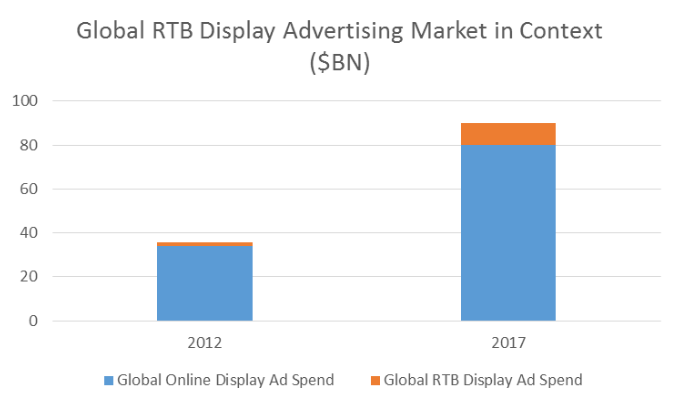
\includegraphics[width=\columnwidth]{rtbmarket.png}
\caption{Global RTB Display Advertising Market in Context}
\label{fig:rtbmarket}
\end{figure}

The core of computational advertising is to find the \textit{optimal match} between \textit{advertisement} and \textit{users}, in some certain context \cite{balakrishnan2014real}. For the advertisers, a major concern is that whether their investments in online advertisement, like other business investments, can be paid back, namely the Return of Investment (ROI). To specify, the profit can be represented as:\
\begin{equation}
profit = PV * CTR * ACP
\end{equation}
Which is the realization formulation for sponsored search, \PV means \textit{Page View}, representing the volumes of retrieved ads, this is the upper bound of cash realization for advertising company, decided by the user experience of the recommended advertisements. \CTR means \textit{Click Through Rate}, it shows the average number of clicks for each advertisement impression, measuring the average click contribution for a single advertisement. specifically, \CTR demonstrates the probability that one advertisement can be clicked, measuring the accuracy of pushed advertisement to the audience, whether the recommended advertisement satisfies the user experience. \ACP means \textit{Average Click Price}, which can be obtained by \(Total Cost / Total Clicks\). It is not surprising that PV, which is decide by the market share of the company and user experience and ACP, which is decided by the company's strategy, are always fixed, therefore, in order to increase the ROI, predicting the CTR will be the crucial technology for advertisement and search engine companies, we can say that the CTR prediction one of the most important part of the realization system of a company, which can be calculated by :
\begin{equation}
CTR = \frac{Clicks}{Impression} \times 100\%
\end{equation}
The key actors for CTR prediction problem can be shown in Figure ~\ref{fig:ctr}
\begin{figure}[h]
\centering
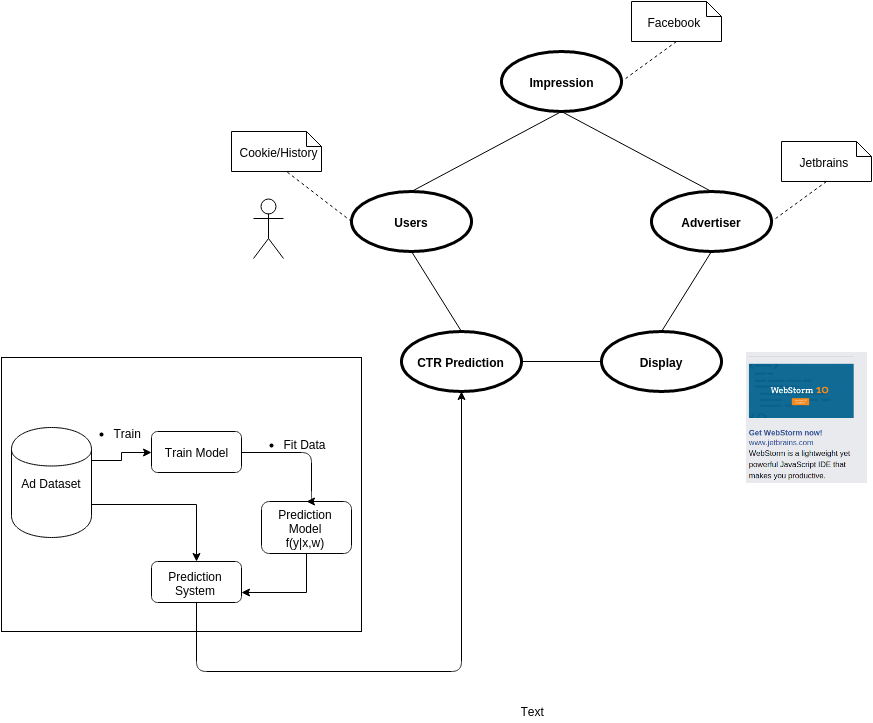
\includegraphics[width=\columnwidth]{ctr1.png}
\caption{CTR prediction Problem}
\label{fig:ctr}
\end{figure}
The challenges of the CTR prediction problem are various, firstly, as we have enterred the age of big data, hundreds of billiions are presented every day \cite{lohr2012age}, many companies have already started the research on large-scale CTR prediction system, such as Google \cite{mcmahan2013ad}, Microsoft \cite{graepel2010web}, Baidu \cite{liu2012enlister} and Facebook \cite{he2014practical}. The problems they want to solve are similar to the challenges for big data, namely the \textit{3V} problem
\begin{itemize}
  \item Volume : The exponential growth in the data storage for online advertisement. Everyday billions of advertisements will be presented with more than a billion feature, unbalanced categories and huge data noise
  \item Velocity : The Ad data evolves a lot every second and the user behaviors change dramatically. CTR changes with time goes, there are always new campaigns and old campaigns will expire.
  \item Variety : Advertisement data are from multiple sources, features are distinct for different campaigns, features are high dimensional and follow non-linear relations.
\end{itemize}
Therefore, the current online RTB advertising system must be able to handle the \textit{ZB-level, relatime } and \textit{high complexity} ad data. Models have to be trained and updated frequently and the strategies must be updated accordingly. 
The normal CTR prediction process can be represented as shown as follows :
\begin{figure}[h]
\centering

\includegraphics[width=\columnwidth]{system.png}
\caption{Machine Learning Process of CTR Prediction}
\label{fig:system}
\end{figure}

Currently, most of the researches are based on how to build a better model and algorithms, however, as said in \cite{facebook2015}, in terms of the efforts of improving the performance of Machine Learning application, the significance of the three core factors are \(Data > Features > Algorithms\). The quality of data itself and the generated decides the upper bound of the performance of CTR prediction problem, however a better algorithm and model can only help reach this upper bound as near as possible. So in this paper I will refocus on the \textit{Feature Generation}, or \textit{Feature Engineering} which are rarely discussed but only in a few literatures and blogs, such as \cite{featureengineering}, and \cite{featureengineeringmeituan}. Based on existing unstructured and complex advertisements, better generated features will help reduce the complexity of model training and \textit{cold start} problem. The new features should have the following characters:
\begin{itemize}
  \item Low Dimensionality : With the explosion of data volume, the number features will grow extremely, without feature engineering, the feature numbers will follow a linear relation with the impression number, as \(O(n)\), \(n\) is the number of impressions in the advertisement dataset. Since for giant companies, like Google or Facebook, each day more than 100 billion impressions of ad data will be generated and distributed storing on thousands machines, we can imagine the astronomical number of features which will be trained and stored, currently, one-hot features are commonly used to generate discrete binary features, for example, image a company owns three types of features, which are \textit{User-related},\textit{Publisher-related} and \textit{Advertiser-related}, in each type there are 10 different categories, such as \textit{region},\textit{publisher network}, \textit{advertiser network},etc. So in total there are 30 categories for each impression. For a campaign, there are 1,000,000 impressions, since the number of features equals to the number of unique items in this dataset, so according to the situation from AdForm and Ipinyou dataset, 5,000,000 will be a possible number of features, an impression vector will look like:
\begin{equation}
 \Big[\underbrace{[0,0,1....0,0,0]}_\textrm{Advertiser Network} + \underbrace{[0,1,0,0,0....0,0,0]}_\textrm{Publisher Network}.... \underbrace{[0,1,0,0....0,0,0]}_\textrm{Region}]
\end{equation}
Therefore, the binary one-hot feature is high dimensional and extremely sparse, and with the new come-in advertisement data, such as the ones from new campaigns, the number of features will also increase accordingly. So it is more efficient to replace the redundant and cumbersome binary feature with the feature with lower and fixed dimensions. 
    \item Scalability : A huge drawback of binary feature is its lack of scalability. Imagine for AdForm the old campaigns are form UK, and the CTR prediction model is trained based on the unique \textit{British Feature}, however, when a new campaign from Netherlands comes in, the overlap between the feature sets of UK old campaigns and Dutch new campaign will be small, at least the category \textit{Region} will be totally different, so the model can be only used for old campaigns and will be abandoned for new ones. Some researches have studied on how to build the model on new campaigns, 
    \item Feature Explainability : Some companies and researchers have turned to deep learning and try to apply this magical method in the field of CTR prediction, such as the slides from \cite{deeplearning} and \cite{wang2014collaborative}, indeed, many companies now run distributed classification system for CTR prediction problems, the data training process has to be finished on Amazon EC2, but on the on hand, the method used well on one computer dose not mean that it will run perfect on distributed system, on the other hand, if deep learning is used, maybe it can improve the performance somewhat, however, firstly, it is hard to implement, secondly, the learned parameters and weights are hard to explain, the parameters of this \textit{Black Box} cannot be interplated with physical meanings.  
    
\end{itemize}

\subsubsection{statistical feature and PCA}

counting feature































\section{Relation Between Counting Feature and Binary Feature Based on Linear Model}
\subsection{Frequency Feature}
\setlength{\parindent}{5ex}

The \textsl{Click Through Rate} (CTR) prediction problem can be characterized as a logistic regression problem. we can use features of ads, terms, and advertisers to learn a model that accurately predicts the CTR for new ads. To train the prediction model, we firstly define the following symbols for later explanations.\vspace{5mm}
The training dataset contains number of \textsl{N} instances, which are the records in datalog containing \textsl{M} fields of user, advertiser and publisher information, as well as their clicking information for each ad impression. The result of the impression, namely whether the user clicks on the ad will be represent by \textsl{y}. Even though normally we use logistic regression to train the model since the dependent variable is dichotomous, here the liner regression is used to prove the relation between model built by \(x_{\text{counting}}\) representing the data instances encoded into \textsl{Counting Feature} and model built by \(x_{\text{binary}}\) representing the data instances encoded into one-hot \textsl{Binary Feature}. The dimension of \(x_{\text{counting}}\) is the number of fields \textsl{M} well the dimension of \(x_{\text{binary}}\) is represend by \textsl{D} for which \(D >> M\). The more detailed information about symbols are shown in Table 1.
\iffalse
\begin{itemize}
\item  Binary Features : \(x_{\text{binary}(N\times D)}\)
\item  Counting Feature : \(x_{\text{counting}(N\times D)}\)
\item  Clicking result : \(y_{(1\times N)}\)
\item  Weights vector of Binary Feature : \(w_{\text{binary}(1\times D)}\)
\item  Weights vector of Counting Feature: \(w_{\text{counting}(1\times M)}\)
\item  Transform Binary Feature to Counting Feature matrix : \(T_{(M\times D)}\)
\item  Calculating feaquency matrix : \(A_{(N\times 1)}\) which is an all-one vector 
$\vec{1 }$  
\item  Field  matrix : \(C_{(M\times D)}\) which is a 0-1 matrix concatenated with \textsl{}{M} vectors \(V_{m,(m = 1...M)}\) and in each vector \(V_m\) only its corresponding positions in field \textsl{m} is filled with 1, with other positions 0.
\item  Diag function : Transform the column vector into a diagonal matrix.\vspace{5mm} 

\end{itemize}
\fi
 It can be proven that 
\[ T = C\times Diag(x_{b}A) \]
The formation of \textsl{T} is 

$$
\begin{pmatrix} 
\vec{F_1} \\
\vec{F_2} \\
.\\
\vec{F_M}

\end{pmatrix}
$$

\noindent in which \($$\vec{F_m}$$ = $$\begin{pmatrix} 
$$\vec{0 }$$ , f_{m1}, f_{m2}, ...f_{mi}... , f_{mI} ,$$\vec{0 }$$ 
\end{pmatrix}$$\), and \(f_{mi}\) represents the occurrence of \(i_{th}\) binary feature in the field \textsl{m} in the whole dataset.\vspace{5mm}

\noindent Next, the relations between \(w_{\text{binary}}\) and \(w_{\text{counting}}\) are proven as follows. 

\begin{equation}
w_{\text{b}} \times x_{\text{b}}^T = y 
\end{equation}

\begin{equation}
(w_{\text{b}}^T \times w_{\text{b}}) \times x_{\text{b}}^T = w_{\text{b}}^T \times y 
\end{equation}

\begin{equation}
x_{\text{b}}^T = (w_{\text{b}}^T \times w_{\text{b}})^{-1} \times w_{\text{b}}^T \times y 
\end{equation}

Using SVD, we can derive that,

\begin{equation}
(w_{\text{b}}^T \times w_{\text{b}})^{-1} \times w_{\text{b}}^T = (w_{\text{b}})^{-1(left)}  
\end{equation}

So we can get that 
\begin{equation}
x_{\text{b}}^T =  (w_{\text{b}})^{-1(left)} \times y 
\end{equation}

We define
\begin{equation}
T = C \times Diag(x_{\text{b}}^T \times A)
\end{equation}


Multiply each size by \textsl{T}, we can get
 
\begin{equation}
T \times x_{\text{b}}^T =  T \times (w_{\text{b}})^{-1(left)} \times y 
\end{equation}

It can be proven that 
\begin{equation}
T \times x_{\text{b}}^T =  x_{\text{c}}
\end{equation}

So
\begin{equation}
x_{\text{c}} =  T \times (w_{\text{b}})^{-1(left)} \times y 
\end{equation}

Since \(T \times (w_{\text{b}})^{-1(left)}\) is a \(M \times 1\) matrix, so multiplying its transposition we can get a constant scalar, 
\begin{equation}
(T \times (w_{\text{b}})^{-1(left)})^T \times (T \times (w_{\text{b}})^{-1(left)}) = \lambda
\end{equation}

So, 
\begin{equation}
1/{\lambda} \times (T \times (w_{\text{b}})^{-1(left)})^T \times x_{\text{c}} =  y
\end{equation}

In conclusion, we can get
\begin{equation} \label{eq:12}
\begin{split}
w_{\text{c}} & =\ 1/{\lambda} \times (T \times (w_{\text{b}})^{-1(left)})^T \\
& = \ 1/{\lambda} \times (C \times Diag(x_{\text{b}}^T \times A) \times (w_{\text{b}})^{-1(left)})^T
\end{split}
\end{equation}

\subsection{Average CTR feature}

\setlength{\parindent}{5ex}

In this section, the relation between  \(w_{\text{ctr}}\) and \(w_{\text{binary}}\) will be deduced, the steps are similar except for specific part of CTR calculating. \vspace{3mm}

Initially, we can get the similar deduction process, 
\begin{equation}
w_{\text{b}} \times x_{\text{b}}^T = y 
\end{equation}

\begin{equation}
(w_{\text{b}}^T \times w_{\text{b}}) \times x_{\text{b}}^T = w_{\text{b}}^T \times y 
\end{equation}

\begin{equation}
x_{\text{b}}^T = (w_{\text{b}}^T \times w_{\text{b}})^{-1} \times w_{\text{b}}^T \times y 
\end{equation}

\begin{equation}
(w_{\text{b}}^T \times w_{\text{b}})^{-1} \times w_{\text{b}}^T = (w_{\text{b}})^{-1(left)}  
\end{equation}

\begin{equation}
x_{\text{b}}^T =  (w_{\text{b}})^{-1(left)} \times y 
\end{equation}

However, then in order to count the number of \textsl{clicks} for each instance, we redefine the transformation matrix \textsl{T} as following, 

\begin{equation}
T_{\text{click}} = C \times Diag(x_{\text{b}}^T \times y)
\end{equation}



From section 1, we can know that, 
\begin{equation}
T_{\text{frequency}} = C \times Diag(x_{\text{b}}^T \times A)
\end{equation}

Since it is easy to know that,

\begin{equation}
(Diag(T_{\text{click}}) \times (1/T_{\text{frequency}} )^T =  T_{\text{ctr}}
\end{equation}

Similar to section 1, we can multiply \(T_{\text{ctr}}\) by both sides of equation (17)

\begin{equation}
T_{\text{ctr}} \times x_{\text{b}}^T =  T_{\text{ctr}} \times (w_{\text{b}})^{-1(left)} \times y 
\end{equation}

It can be proven that 

\begin{equation}
T_{\text{ctr}} \times x_{\text{b}}^T =  x_{\text{ctr}}
\end{equation}

So,

\begin{equation}
 x_{\text{ctr}} =  T_{\text{ctr}} \times (w_{\text{b}})^{-1(left)} \times y 
\end{equation}

It is similar to section 1 that \(T_{\text{ctr}} \times (w_{\text{binary}})^{-1(left)}\)is a \(M \times 1\) matrix, so we define, 
\begin{equation}
(T_{\text{ctr}} \times (w_{\text{b}})^{-1(left)})^T \times (T_{\text{ctr}} \times (w_{\text{b}})^{-1(left)}) = \lambda
\end{equation}

So, 
\begin{equation}
1/{\lambda} \times (T_{\text{ctr}} \times (w_{\text{b}})^{-1(left)})^T \times x_{\text{ctr}} =  y
\end{equation}

In conclusion, we can get
\begin{equation} 
\begin{split}
w_{\text{ctr}} & =\ 1/{\lambda} \times (T_{\text{ctr}} \times (w_{\text{b}})^{-1(left)})^T \\
& = \ 1/{\lambda} \times (Diag(T_{\text{click}}) \times (1/T_{\text{frequency}} )^T \\ 
& \times (w_{\text{b}})^{-1(left)})^T \\
& = \ 1/{\lambda} \times (Diag(C \times Diag(x_{\text{b}}^T \times y)) \\ 
& \times (1/ (C \times Diag(x_{\text{b}}^T \times A) )^T) \times (w_{\text{b}})^{-1(left)})^T
\end{split}
\end{equation}

\subsection{Non-linearity of Counting Feature}
We define the non-linear formulation of logistic regression as follows:
\begin{equation}
Pr(w_{\text{i}}|x_{\text{i}}) = Bern_{w_{\text{i}}}[sig(a_{\text{i}})]
\end{equation}

in which \(sig(a_{\text{i}})\) is the sigmoid function and the activation \(a_{\text{i}}\) is given by,

\begin{equation}
a_{\text{i}} = \Phi^T f(x_{\text{i}})
\end{equation}

and \(f(x)\) is the nonlinear transformation of the space \(x\). 
In our case, we can regard \(f(x)\) as the transformation matrix \(T\) which transform the binary feature space into the counting feature space, then in our case of frequency feature and average CTR feature, the weights space should be derived as \(\Phi^T \) and its value should be decided by the relations in last two paragraphs. So we successfully transform the linear logistic regression on \(N\) dimension to the incremental fitting and boosting problem, we will do some experiment to prove the equivalence of them.

Also, 
\begin{figure}[h]
\centering
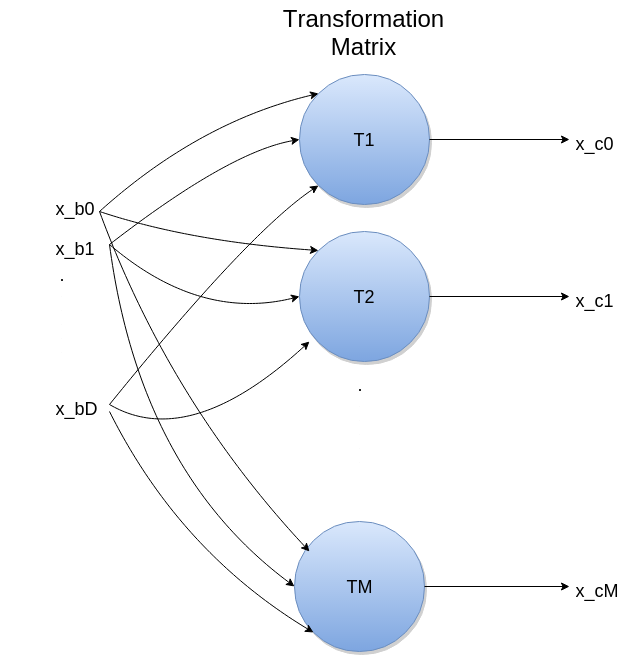
\includegraphics[width=\columnwidth]{countingfeature.png}
\caption{Binary Feature to Counting Feature}
\label{fig:counting}
\end{figure}

from linear to nonlinear transformation 

From above knowledge we already know that counting feature is a statistical representation of binary feature, which compress the information of the whole dataset, and counting feature can reduce the high dimension of binary feature to lower dimensions, namely from millions of dimensions to less than 1 thousand. The cost of this reduction is assuming that binary feature follows a linear model to the label, such a space transformation will lead to the non-linearity of the counting feature. So we have to use non-linear regression model, such as GBDT to solve this problem. Using the mothod in \cite{he2014practical}, one way to do so is to transform the input space so that the non-linearity is eliminated and a linear feature space can be obtained, this can be done by GBDT, and according to \cite{cover1965geometrical}:

\textit{"A complex pattern-classification problem, cast in a high-dimensional space nonlinearly, is more likely to be linearly separable than in a low-dimensional space, provided that the space is not densely populated."}

So the counting feature can be trained into the model when following a non-linear regression model to eliminate the non-linearity meanwhile obtain the comparable performance in terms of CTR prediction with binary feature.

\section{Counting Feature Generation and Anaysis in Advertisement Cold Start Problem}
In this part, the cold start problem will be discussed. Now the experiment is done in which the placement id is counted and when the clicks in one palcement id's corresponding is higher than 200, the instances will be remained, and the overlap of placement id in the train dataset and test dataset will be filtered out. Then for the training dataset all the campains in the test dataset are new. Many experiments are done now but result is confused. Generally the result is as follows: 

Performance of Binary Feature in cold start > Counting Feature with update weights using new coming data > Counting feature without update weights using weights from previous campains > Binary feature without update weights


I am trying to figure out the reason why binary feature performs well in cold start problem and it seems biased dataset is a cause and I try to split the model into generic and specific parts and overcome the bias.
\subsection{Model Similarity Analysis}
At first, we will start from the easier one, the frequency feature. Let's assume that we have two datasets, dataset \(Dataset_{\text{1}}\) and \(Dataset_{\text{2}}\), for each dataset we can get \(w_{\text{counting}}\) and \(w_{\text{binary}}\) respectively. Let's abbreviate them as \(w_{\text{c1}}\) and \(w_{\text{b1}}\) as well as \(w_{\text{c2}}\) and \(w_{\text{b2}}\). 

From \ref{eq:12} we can get the following equation:
\begin{equation} \label{eq:28}
\begin{split}
w_{\text{counting}} & =\ 1/{\lambda} \times (C \times Diag(x_{\text{binary}}^T \times A) \times (w_{\text{binary}})^{-1(left)})^T \\
& = \ 1/{\lambda} \times (C \times Diag(x_{\text{binary}}^T \times A) \times ((w_{\text{binary}}^T \times w_{\text{binary}})^{-1} \\
& \times w_{\text{binary}}^T )^T
\end{split}
\end{equation}

We will make use of cos similarity, which is used to measure the distance between two vectors to measure the similarity of two \(w_{\text{counting}}\) from \(Dataset_{\text{1}}\) and \(Dataset_{\text{2}}\). The formation of similarity can be shown as follows:

\begin{equation} \label{29} 
\begin{split}
Similarity & = \cos(\Theta) = \frac{w_{\text{c1}} \times w_{\text{c2}}^T} {||w_{\text{c1}}|| \times ||w_{\text{c2}}|| }
\end{split}
\end{equation}

Substitute \(w_{\text{c1}}\) with \ref{eq:12} and represent \(Diag(x_{\text{binary}}^T \times A)\) using \(Diag(f)\) since this diagonal entries \(d(i,i) \) shows the frequency of feature \(i\), we can get the following equation:


\begin{equation} \label{30} 
\begin{split}
\frac{w_{\text{c1}} \times w_{\text{c2}}^T} {||w_{\text{c1}}|| \times ||w_{\text{c2}}|| } & =  \frac{w_{\text{c1}} \times w_{\text{c2}}^T} {\sqrt{w_{\text{c1}} \times w_{\text{c1}}^T} \times \sqrt{w_{\text{c1}} \times w_{\text{c2}}^T} }
\end{split}
\end{equation}

To simply, at first we will deduct the following equation:

\begin{equation} \label{31} 
\begin{split}
w_{\text{ci}} \times w_{\text{cj}}^T & = \frac{1}{{\lambda}_{i}{\lambda}_{j} } \times (w_{\text{bi}} \times Trans_{i}) \times (w_{\text{bj}} \times Trans_{j})^T \\
& subject : (i.j = 1 \cup 2)
\end{split}
\end{equation}


In which \(Trans\) is a Transformation Matrix, 
\begin{equation} \label{31} 
\begin{split}
Trans = ((w_{\text{binary}}^T \times w_{\text{binary}})^{-1})^T \times (Diag(f))^T \times C^T  
\end{split}
\end{equation}

Then, we will focus on the transformation matrix. 

Since \(((w_{\text{binary}}^T \times w_{\text{binary}})^{-1})^T\) is a symmetric matrix, so it equals to its own transposition. 


